\section{Technical Implementation}
\label{section:techimpl}
This section describes the current solution, the implemented software architecture and the final results of the project.
Discrepancies between the planned implementation approach and the current solution are listed in \sectionref{section:techimpl:comparison_impl}.

\subsection{Meteoblue Integration}
\label{section:techimpl:meteoblue}
While the bachelor project specifictation document described the use of \emph{meteoblue}'s "basic 1h" package, this was not the only package that was used in the final implementation.
After the cancellation of the technical interview with \emph{meteoblue} and further research into additional, available weather data sources, the package "clouds 1h" was suggested.
It provides an overview of cloud coverage percentage for each cloud layer, which is exactly what the implementation was missing.
\emptyline
\begin{tabularx}{\linewidth}{|l|X|}
    \hline
    \textbf{Package name}   & \textbf{Description} \\ \hline
    Basic (1h)              & Mainly used for shading and visual effects. \\ \hline
    Clouds (1h)             & Mainly used for cloud coverage data. \\ \hline
\end{tabularx}
\emptyline
The following table displays a list of properties from both data packages and how they are used in the final implementation.
\emptyline
\begin{tabularx}{\linewidth}{|l|l|X|}
    \hline
    \textbf{Property name}      & \textbf{Source}     & \textbf{Usage}                                 \\ \hline
    Wind speed                  & Basic (1h)          & Used with a multiplier                         \\ \hline
    Wind direction              & Basic (1h)          & Converted form degrees to a directional vector \\ \hline
    Precipitation               & Basic (1h)          & Used for controlling rain particle system and cloud color.\newline Factored into cloud edge highlight colors from sunshine.\newline Factored into skybox colors. \\ \hline
    Precipitation probability   & Basic (1h)          & Included in approximation of precipitation     \\ \hline
    Cloud coverage low          & Clouds (1h)         & Used unmodified                                \\ \hline
    Cloud coverage mid          & Clouds (1h)         & Used unmodified                                \\ \hline
    Cloud coverage high         & Clouds (1h)         & Used unmodified                                \\ \hline
\end{tabularx}
\emptyline
Other properties like temperature and UV index provide insufficient or irrelevant information and have therefore not been mapped.

\clearpage

\subsection{ArcGIS Integration}
\label{section:techimpl:arcgis}
During the research phase of the project, the \emph{ArcGIS Maps SDK for Unity} \cite{arcgis:unitysdk} was found. This proved to be a suitable replacement for the originally planned \emph{swisstopo} elevation model data.
The plugin was easily installed. The setup process required minimal amount of effort and the plugin was ready to run in no time. 

\begin{figure}[H]
    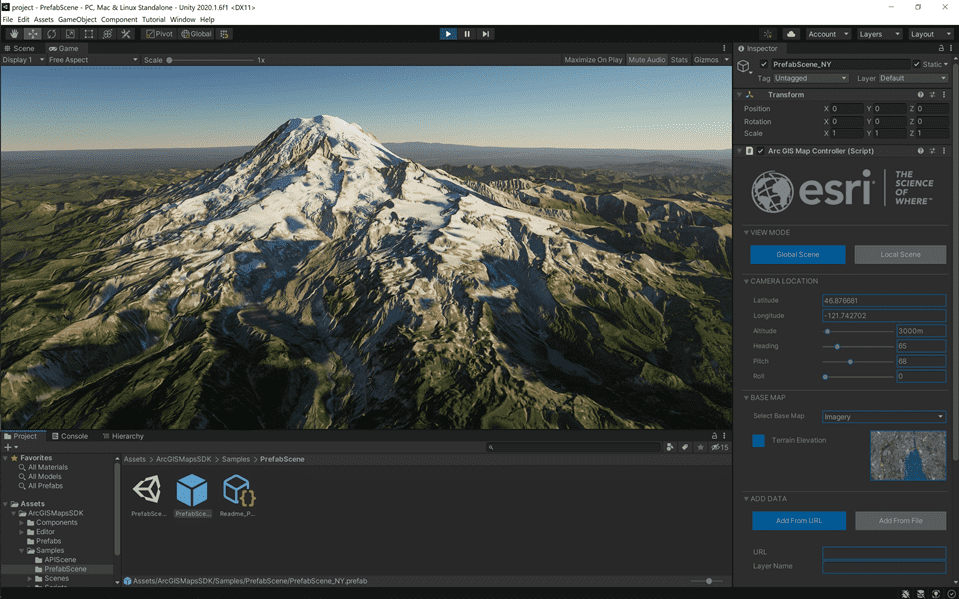
\includegraphics[width=\linewidth]{unity-sdk.png}
    \caption{ArcGIS Maps SDK for Unity \protect\cite{arcgis:unitysdk}.}
\end{figure}

\noindent
After setting up the plugin in Unity, the camera needed to be positioned on top of the Gurten mountain. Also, there needed to be a translation mechanic to move the camera to the top of the Bantiger mountain.
This was done with via script and is not part of the \emph{ArcGIS} plugin.

\subsection{Shader Architecture}
\label{section:techimpl:architecture}
The architecture described in the implementation approach in \sectionref{section:impl:layers} was chosen, but underwent some alterations.
First, 

\subsection{Noise Generation}
\label{section:techimpl:noise}

\subsection{Shadow Casting}
\label{section:techimpl:shadow}

\subsection{Results}
\label{section:techimpl:results}

\subsection{Testing}
\label{section:techimpl:testing}

\subsection{Measurability}
\label{section:techimpl:measure}

\subsection{Comparison to Implementation Approach}
\label{section:techimpl:comparison_impl}

\subsection{Comparison to Previous Work}
\label{section:techimpl:comparison}
%performance

2. technical impl: algorithms, progress pics, 
2. results: what has been achieved, how realistic, compare to spec
2. testing: 1-2 paragraphs, visual testing, gui stuff, messbarkeit,
